% VUT FIT MITAI
% MSZ 2021/2022
% Author: Vladimir Dusek
% Login: xdusek27

%%%%%%%%%%%%%%%%%%%%%%%%%%%%%%%%%%%%%%%%%%%%%%%%%%%%%%%%%%%%%%%%%%%%%%%%%%%%%%%%

\chapter{Hledání nejkratších cest ze zdrojového uzlu do všech ostatních uzlů grafu (Bellman-Fordův algoritmus, Dijkstrův algoritmus).}

%%%%%%%%%%%%%%%%%%%%%%%%%%%%%%%%%%%%%%%%%%%%%%%%%%%%%%%%%%%%%%%%%%%%%%%%%%%%%%%%

\section{Metadata}

\begin{itemize}
    \item Předmět: Grafové algoritmy (GAL)
    \item Přednáška:
    \begin{itemize}
        \item 7) Nejkratší cesty z jednoho vrcholu, Bellman-Fordův algoritmus, nejkratší cesta z jednoho vrcholu v orientovaných acyklických grafech.
        \item 8) Dijkstrův algoritmus. Nejkratší cesty ze všech vrcholů.
    \end{itemize}
    \item Záznam:
    \begin{itemize}
        \item 2020-11-05
    \end{itemize}
\end{itemize}

%%%%%%%%%%%%%%%%%%%%%%%%%%%%%%%%%%%%%%%%%%%%%%%%%%%%%%%%%%%%%%%%%%%%%%%%%%%%%%%%

\section{Úvod a kontext}

\textit{Viz. \uv{Úvod a kontext} v předchozí otázce.}

\paragraph*{Cena cesty} Nechť $G = (V, E)$ je ohodnocený graf s váhovou funkcí $w: E \mapsto \mathbb{R}$. Cena cesty $p = \langle v_o, v_1, \dots, v_k \rangle$ je suma $$
w(p) = \sum_{i=0}^k w(v_i, v_{i+1})
$$.

\paragraph*{Cena nejkratší cesty} Cena nejkratší cesty z $u$ do $v$ je $$
\delta(u, v) = \begin{cases}
    min( \{ w(p) : u \xRightarrow{\text{p}} v \} ) \\
    \infty ~ \text{pokud cesta neexistuje}
\end{cases}
$$.

\paragraph*{Nejkratší cesta} Nejkratší cesta z $u$ do $v$ je pak libovolná cesta $p$ taková, že $w(p) = \delta(u, v)$.

\paragraph*{Cena cesty se záporným cyklem} Pokud na cestě z $u$ do $v$ existuje záporný cyklus (cyklus jehož celková cena je záporná), pak $\delta(u, v) = - \infty$.

\paragraph*{Záporné ohodnocení hran} Pokud na cestě z $u$ do $v$ neexistuje záporný cyklus, tak algoritmy pracují dobře i se záporným ohodnocením hran.

\paragraph*{Reprezentace cesty} Cestu reprezentujeme pomocí pole předchůdců $\pi$.

\paragraph*{Hledání nejkratších cest ze všech uzlů do jednoho} Tento problém lze řešit stejnými algoritmy. Graf se transponuje, provede se algoritmus pro problém \uv{hledání nejkratších cest ze jednoho uzlu do všech ostatních uzlů} a poté se transponuje zpět.

%%%%%%%%%%%%%%%%%%%%%%%%%%%%%%%%%%%%%%%%%%%%%%%%%%%%%%%%%%%%%%%%%%%%%%%%%%%%%%%%

\section{Pomocné funkce}

\noindent\begin{minipage}{\linewidth}
\begin{lstlisting}[language=Python, caption={Pomocná inicializační funkce.}]
def initialize_single_source(G, s):
    # G je graf
    # s je vychozi uzel
    for v in G.V:
        d[v] = INF  # d je pole vzdalenosti
        pi[v] = NULL  # pi je pole predchudcu
    d[s] = 0
\end{lstlisting}
\end{minipage}

\noindent\begin{minipage}{\linewidth}
\begin{lstlisting}[language=Python, caption={Pomocná funkce \textit{relax}.}]
def relax(u, v, w):
    # u a v jsou uzly grafu
    # w je vahova funkce
    if d[v] > d[u] + w(u, v):
        d[v] = d[u] + w(u, v)
        pi[v] = u
\end{lstlisting}
\end{minipage}

\begin{figure}[H]
    \centering
    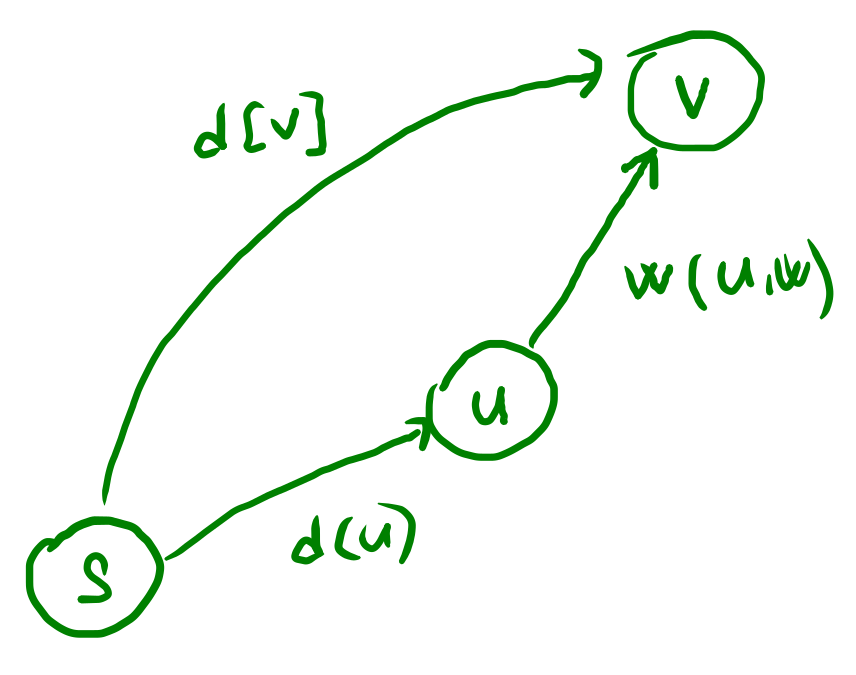
\includegraphics[width=0.4\linewidth]{46/relax.png}
    \caption{Ukázka činnosti funkce \textit{relax}.}
\end{figure}

%%%%%%%%%%%%%%%%%%%%%%%%%%%%%%%%%%%%%%%%%%%%%%%%%%%%%%%%%%%%%%%%%%%%%%%%%%%%%%%%

\section{Bellman-Fordův algoritmus}

Slouží pro řešení v obecných grafech (mohou obsahovat cykly a záporné hrany).

\bigskip\noindent\begin{minipage}{\linewidth}
\begin{lstlisting}[language=Python, caption={Algoritmus Bellman-Ford.}]
def bellman_ford(G, s, w):
    # G je graf
    # s je vychozi uzel
    # w je vahova funkce

    # faze inicializace
    initialize_single_source(G, s)
    n = len(G.V) # pocet uzlu

    # faze relaxace: provedeni n * (n-1) relaxaci
    for _ in range(0, n-1):
        for u, v in G.E:
            relax(u, v, w)

    # faze detekce zaporneho cyklu
    for u, v in G.E:
        if d[u] > d[v] + w(u, v):
            return NULL

    return d, pi
\end{lstlisting}
\end{minipage}

%%%%%%%%%%%%%%%%%%%%%%%%%%%%%%%%%%%%%%%%%%%%%%%%%%%%%%%%%%%%%%%%%%%%%%%%%%%%%%%%

\section{Dijkstrův algoritmus}

Slouží pro řešení v acyklických grafech bez záporných hran. Pro takto omezený problém existují rychlejší algoritmy než pro problém v obecných grafech.

\bigskip\noindent\begin{minipage}{\linewidth}
\begin{lstlisting}[language=Python, caption={Algoritmus Dijkstra.}]
def dijkstra(G, s, w):
    # G je graf
    # s je vychozi uzel
    # w je vahova funkce

    # faze inicializace
    initialize_single_source(G, s)
    Q = Queue(G.V) # prioritni fronta uzlu

    # faze relaxace
    while not Q.empty():
        u = Q.extract_min(d) # vrati prvek z Q s nejmensi hodnotou v d

        # pro vsechny sousedy uzlu u (Adj je seznam sousedu)
        for v in Adj[u]:
            relax(u, v, w)

    return d, pi
\end{lstlisting}
\end{minipage}
